\section{S'en protéger}


\frame{\tableofcontents[currentsection]}


\begin{frame}

Quelques solutions pour se protéger des failles CSRF:
\\
\begin{itemize}
\item Ne pas faire d'actions potentiellement dangereuses avec GET
\item Utiliser un token d'authentification
\item Renseigner le header HTTP 'Referrer' et le vérifier coté serveur
\item Supprimer ses cookies le plus souvent possible
\end{itemize}

Une faille XSS rendrait obsolète la plupart de ces méthodes de protection.

\end{frame}

\begin{frame}
\begin{block}{Synchronizer token pattern}
\begin{itemize}
\item Token unique généré par session d'utilisateur ou même par requête
\item Cryptographiquement sûr (graine aléatoire, session id, timestamp, ...)
\item Inséré dans tous les formulaires modifiant l'état du serveur
\item Vérifié par le serveur à chaque requête
\end{itemize}
\end{block}
\end{frame}

\begin{frame}
\centerline{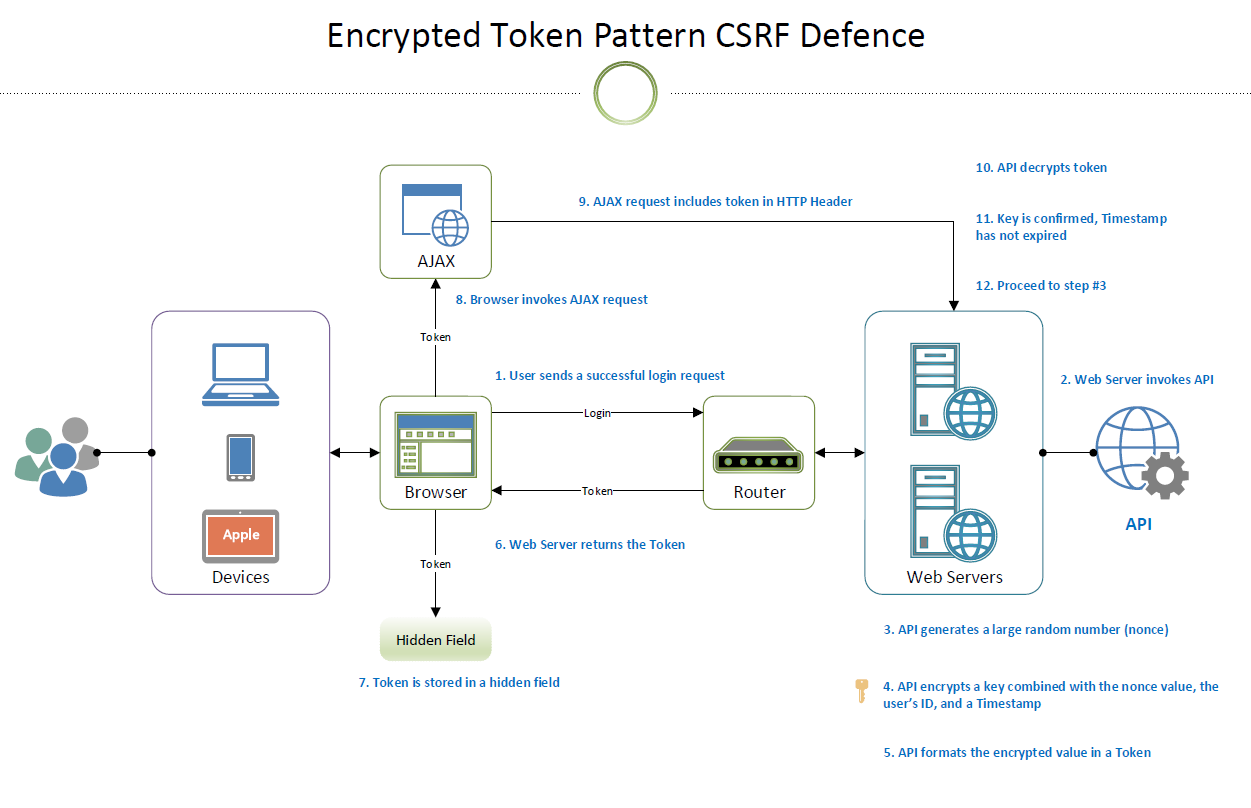
\includegraphics[scale=0.35]{encrypted-token-pattern.png}}
\end{frame}

\begin{frame}
\begin{block}{Inclusion du token dans un formulaire}
\lstinputlisting[language=HTML]{form-token.html}
\end{block}
\end{frame}

